\documentclass[conference]{IEEEtran}
\usepackage{graphicx}
\usepackage{algorithm}
\usepackage{algorithmic}

\makeatletter
\def\BState{\State\hskip-\ALG@thistlm}
\makeatother


\begin{document}
\title{Assignment 5 - Finding accurate Value Of $\log{\left(\frac{x}{x-1}\right)}$ Using Series Expansion}

\author{\IEEEauthorblockN{Parag Parihar}
\IEEEauthorblockA{Roll No:- IIT2016095\\
iit2016095@iiita.ac.in}
\and
\IEEEauthorblockN{Rakshit Sai}
\IEEEauthorblockA{Roll No:- IIT2016126\\
iit2016126@iiita.ac.in}
\and
\IEEEauthorblockN{Adarsh Agrawal}
\IEEEauthorblockA{Roll No:- IIT2016516\\
iit2016516@iiita.ac.in}
\and
\IEEEauthorblockN{Nilotpal Pramanik}
\IEEEauthorblockA{Roll No:- IRM2016501\\
irm2016501@iiita.ac.in}
\thanks{Manuscript received February 2, 2018.}}

\markboth{Assignment-1, IDAA432C; B.Tech.(IT)}
{Shell \MakeLowercase{\textit{et al.}}: Bare Demo of IEEEtran.cls for Journals}

\maketitle

\IEEEpeerreviewmaketitle
\begin{abstract}
 Write an efficient algorithm to calculate the value of $\log{\left(\frac{x}{x-1}\right)}$ for some given input value of x by repeatedly exploring and adding the successive terms in the expansion of the series $\log{\left(\frac{x}{x-1}\right)}$ = $\frac{1}{x}$+$\frac{1}{2x^2}$+$\frac{1}{3x^3}$ + ... .Termination condition is $|S_{i}$ - $ S\textsubscript{i-1}| \leq \epsilon $, where $S_{x}$ denotes value of the series computed up to the $ x\textsuperscript{th}$ term and $\epsilon$ is an arbitrarily small positive number also taken as an user input for your algorithm. Plot time complexity vs. $\epsilon$ Also plot no. of terms considered (summed) vs. $\epsilon$ accuracy of the answer produced by your algorithm.
\end{abstract}

\section{\textbf{Introduction and Literature Survey}}
We have to write an efficient algorithm to calculate the value of \textbf{$\log{\left(\frac{x}{x-1}\right)}$} for a given input value of x by repeatedly exploring and adding the successive terms in the expansion of the series $\log{\left(\frac{x}{x-1}\right)}$ = $\frac{1}{x}$+$\frac{1}{2x^2}$+$\frac{1}{3x^3}$ + ... . The termination condition is $|S_{i}$ - $ S\textsubscript{i-1}| \leq \epsilon $ where $S_x$ denotes value of the series computed up to the $ x\textsuperscript{th}$ term and $\epsilon$ is an arbitrarily small positive number also taken as an user input for your algorithm. We need to plot time complexity vs $\epsilon$ and also need to plot no. of terms considered (summed) vs. accuracy of the answer produced by the algorithm.
Along with that, We need to make sure that our algorithm is the best algorithm and the given problem cannot be solved in a much better way than the way we have solved it. We also need to compare it with the previous group which has done the same problem. We need to solve the problem in a much better way than the previous group or we need to prove that it cannot be done in a better way than they have done.
The report contains :-\\
2. Algorithm Design\\
3. Algorithm Analysis\\
4. Experimental Analysis\\
5. Comparison\\
6. Conclusion\\

\section{\textbf{Algorithm Design}}
To construct the algorithm for this particular problem firstly we have to scan the value of \textbf{x} as well as \textbf{e},i.e basically the value of \textbf{$\epsilon$}.And pass these two elements as the attributes of the function named \textbf{Function} and assigned the return value at \textbf{ans}.Then we have assigned the value of $\log{\left(\frac{x}{x-1}\right)}$ to \textbf{original}.As well as the value of $\textbf{ original - ans}$ has been assigned to \textbf{error}.We are calculating the percentage of the error through the formula $\left(\frac{\textbf{original - ans}}{\textbf{original}}\right)*100$ and storing it into the variable \textbf{percentage\_error}.\\

In the function \textbf{Function} we are taking the values of {\textbf{x} and {\textbf{e} as the attributes and there we are initializing the value of the variables \textbf{last} to \textbf{0.0}, \textbf{latest} to the value of $\frac{\textbf{1}}{\textbf{x}}$ and \textbf{product} to \textbf{x} accordingly. After that we are going in to the while loop by satisfying the condition \textbf{latest - last} $>$ $\epsilon$.There we are updating the value of \textbf{product*x} to \textbf{product} as we have to calculate power of \textbf{x} for each iteration , the value at \textbf{latest} to \textbf{last} and the value of \textbf{latest} + $\frac{1}{\textbf{product*i}}$ to \textbf{latest}.We are coming out of the loop by incrementing the value of \textbf{i} which has been already declared as \textbf{2} outside the loop.And after all execution the function \textbf{Function} is returning the value of \textbf{latest} which is value of series expansion to the variable \textbf{ans} declared in the \textbf{Main} function.

\begin{algorithm}[H]
\caption{Function}
\end{algorithm}
\begin{algorithmic}[1]
\STATE \textbf{INPUT: x, $\epsilon$}
\STATE \textbf{OUTPUT: value of series expansion of $\log{\left(\frac{x}{x-1}\right)}$ according to $\epsilon$}
\STATE $ last \gets 0.0 $
\STATE $  latest \gets \frac{1}{x}$
\STATE $ product \gets x $
\STATE $ i \gets 2$ 
\WHILE{ latest - last $>$ $\epsilon$}
	\STATE $product \gets product*x$
    \STATE $ last \gets  latest $
    \STATE $ latest \gets latest + \frac{1}{product*i}$
    \STATE $ i \gets i+1$
\ENDWHILE
\STATE \textbf{return} latest  
\end{algorithmic}


\begin{algorithm}[H]
\caption{Main Function}
\end{algorithm}
\begin{algorithmic}[1]
\STATE \textbf{Scan the value of x where x$>$1 and $\epsilon$}
\STATE $ ans \gets \textbf{function(x,$\epsilon$)} $
\STATE $ original \gets \textbf{Exact value of series} $
\STATE $ error \gets \textbf{ original - ans} $
\STATE $ percentage\_error \gets 
\left(\frac{\textbf{original - ans}}{\textbf{original}}\right)*100$
\end{algorithmic}


\section{\textbf{Analysis and Discussion}}
In this section we have analysed all the cases including  time complexity and  graphs and notations.
\subsection{\textbf{Time-Complexity-------}}
\subsubsection{\textbf{Best-Case}}
The best case for our algorithm consists no iteration of while loop, and this will happen when $\epsilon$ is greater than equal to $\frac{1}{x}$.
In this case no. of instructions are 8 .However this will not give accurate value of series expansion for the given x.\\
\subsubsection{\textbf{Worst-Case}}
The worst case for a given  x would be when $\epsilon$ is just greater than zero i.e when $\epsilon$ is positive and has the least value possible. This is considered to be the worst case because the algorithm will have to calculate values for maximum number of terms.\\ 
The time complexity depends on $\epsilon$ as well as the x given. The bigger the x ,the more number of terms is required to make the required difference less than $\epsilon$. Therefore the worst case is when $\epsilon$ is positive and as small as possible and given x is  as large as possible. The given problem statement asks us to plot time units versus $\epsilon$ for any fixed value of x.
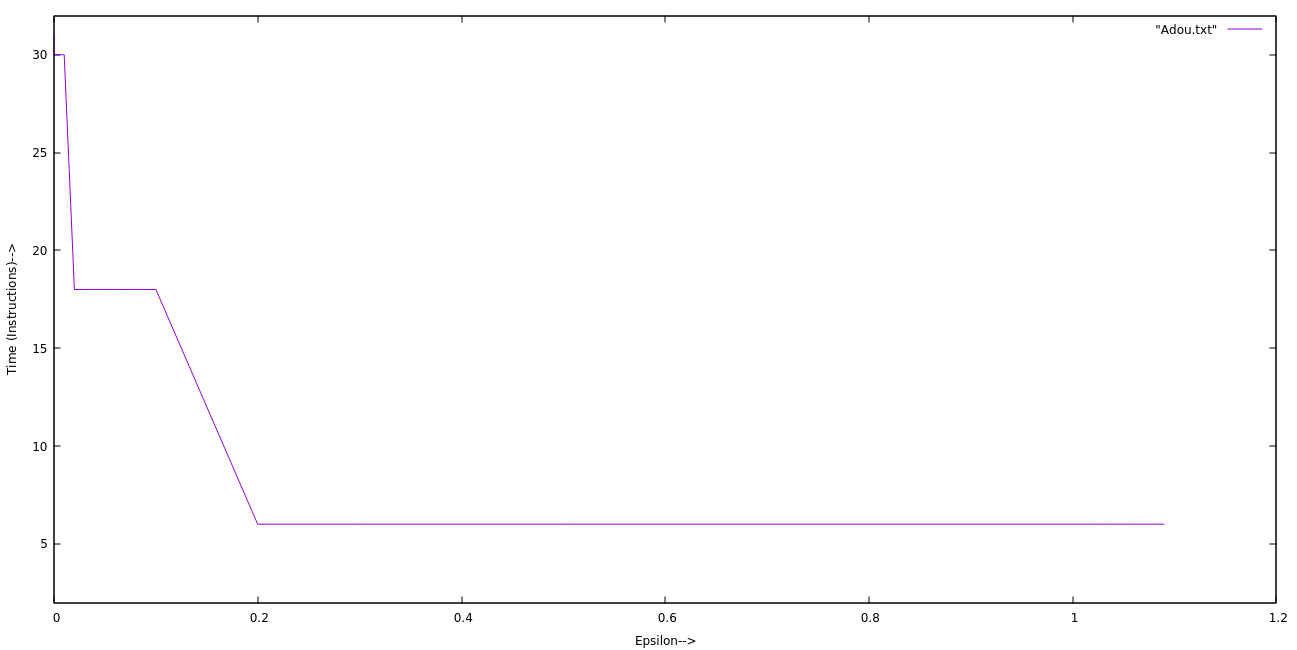
\includegraphics[height =  5.0cm,width = \linewidth]{graph.png}
\textbf{Fig.1 Number of instructions vs $\epsilon$}\\\\
The question asks us to plot the graph between the number of
terms considered and the accuracy percentage. Therefore plotting the number of terms considered and the percentage error would be equivalent.We can see that in the graph as we are increasing no. of terms the error is decreasing drastically. For the following graph we have taken the value of $\epsilon$ 0.
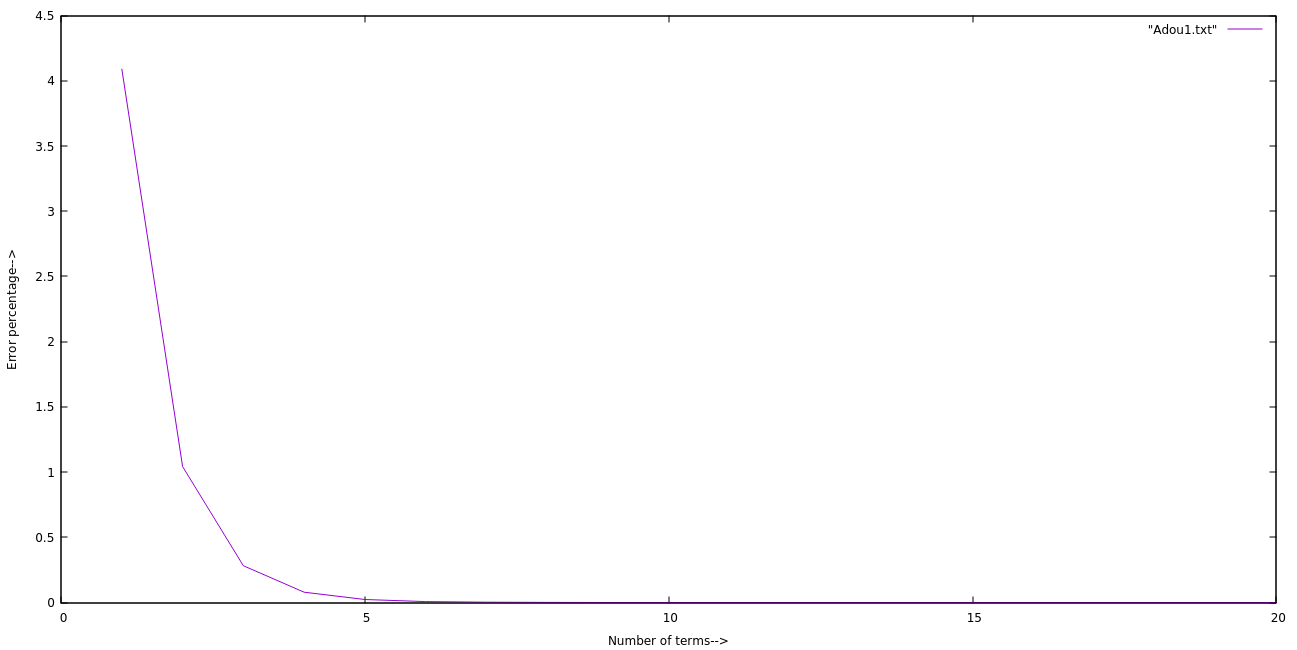
\includegraphics[height =  5.0cm,width = \linewidth]{graph1.png}
\textbf{Fig.2 :  No of terms considered vs  percentage error }\\


\section{\textbf{Experimental Analysis}}
We revised the commands and basic functions of \textbf{GNUPlot} to plot   graphs and other relevant analysis related to our algorithm. While making this report we also learnt the basics of making reports using \textbf{LATEX} in IEEE format using \textbf{IEEEtran} class. \\\\ 
For first graph that is between $\epsilon$ and time , we have taken any random value of x and for different value of $\epsilon$ we have calculated value of time using count in our code. In this way we got following table for $\epsilon$ and time(Instructions) :-\\
\begin{table}[h!]
\begin{center}
    \label{tab:table1}
    \begin{tabular}{|c|c|} % <-- Alignments: 1st column left, 2nd middle and 3rd right, with vertical lines in between
   \hline
     \textbf{$\epsilon$} & \textbf{Instructions}\\
     \hline
      1.02000000  & 6 \\
      \hline
      1.01000000  & 6\\
      \hline
      0.90000000  & 6\\
      \hline
      0.70000000  & 6\\
      \hline
      0.50000000  & 6\\
      \hline
      0.30000000  & 6\\
      \hline
      0.20000000 & 6\\
      \hline
      0.09800000 & 17\\
      \hline
      0.07000000 & 17\\
      \hline
      0.05060000 & 17\\
      \hline
      0.03000000 & 17\\
      \hline
      0.02000000 & 17\\
      \hline
      0.01000000 & 28\\
      \hline
      0.00900000 & 28\\
      \hline
      0.00700000 & 28\\
      \hline
      0.00500000 & 28\\
      \hline
      0.00300000 & 28\\
      \hline
    \end{tabular}
\end{center}
\end{table}
\\
From above table, we can see that as the value of $\epsilon$ is increasing the no. of iterations are increasing but after certain value of $\epsilon$ no. of instruction gets constant value. 

For second graph that is between No. of terms considered vs Percentage Error, we have taken any random value of x and for different no. of iterations we have calculated percentage error In this way we have got following table :- 
\begin{table}[h!]
\begin{center}
    \label{tab:table1}
    \begin{tabular}{|c|c|} % <-- Alignments: 1st column left, 2nd middle and 3rd right, with vertical lines in between
   \hline
     \textbf{No. of Terms} & \textbf{Error}\\
     	\hline
		10 & 0.0000559\\
      	\hline
	  	9 & 0.00018249 \\
      	\hline
		8 & 0.00060016 \\
        \hline
		7 & 0.00199239 \\
        \hline
		6 & 0.00669119 \\
        \hline
		5 & 0.02280134 \\
        \hline
		4 & 0.07918688 \\
        \hline
		3 & 0.28217482 \\
        \hline
		2 & 1.04337959 \\
        \hline
		1 & 4.08819868 \\
      	\hline
    \end{tabular}
\end{center}
\end{table}

\section{\textbf{COMPARISON}}
By comparing the algorithm which we presented with the algorithm designed by the previous group we can tell that the one which we designed is much better and optimized since the complexity of our algorithm is $\textbf{$O(n)$}$ where \textbf{n is no. of iterations (for while loop)}. and that of the other group is $\textbf{$O(n+log(n!)$)}$. The reason the other group have arrived with the time complexity of $\textbf{$O(n+log(n!)$)}$ is that they have used the \textbf{power function} in order to calculate the power of a number which is taking them \textbf{log(i!)} where “ i is the current power of x”,  for each iteration and the power function is in the while loop which is making the loop run until the condition in the loop is satisfied.\\
 As we can understand in our algorithm in each iteration of while loop there is constant no. of instructions (say c) , so our algorithm’s complexity is $O(cn)$ or $O(n)$,   but in other group’s  algorithm, instructions for while loop is like $c+log(2) + c+log(3) + c+log(4) + c+log(5) + . . . . + c+log(n)$, i.e, which is equivalent to $O(nc + log(n!))$  or $O(n + log(n!))$  where \textbf{“c is constant instruction in each iteration”}.  


\section{\textbf{Conclusion}}
In the assignment we have designed an algorithm to find the value of $\log{\left(\frac{x}{x-1}\right)}$ using the \textbf{Taylor’s Series Expansion}. We had to give a value of x and the result will be $\frac{1}{x}$ + $\frac{1}{2x^2}$ + $\frac{1}{3x^3}$ + ... . The expansion length also depends on the value of x. The series must follow the inequality $|S_{i}$ - $ S\textsubscript{i-1}| \leq \epsilon $. Here $S_x$ is the value of the series computed till the xth term and the term $\epsilon$ is very very small and is chosen randomly. Epsilon is taken as the input in the algorithm.\\ We also compared our algorithm with the one which is submitted by the previous group. We have optimized our algorithm even more and the complexity of our algorithm is O(n) where \textbf{n is no. of iterations} .We have also plotted the graph for \textbf{Complexity vs $\epsilon$} and \textbf{Number of terms considered vs the accuracy of the answer produced by the algorithm}.



\begin{thebibliography}{1}
\bibitem{IEEEhowto:kopka}
Introduction To Algorithms (Second Edition) by Thomas H.Cormen,
Charles E.Leiserson , R.L.Rivest and Clifford Stein.
\bibitem{}
The C Programming Language by Brian Kernighan and Dennis Ritchie.
\bibitem{}
https://www.geeksforgeeks.org/
\bibitem{}
https://www.stackoverflow.com/
\end{thebibliography}

\end{document}
